3. $y=\cfrac{x^2+3x}{|x+3|}+x=\begin{cases} 2x,\ x>-3,\\ 0,\ x<-3.\end{cases}$
$$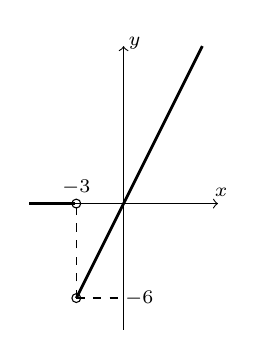
\begin{tikzpicture}[scale=0.2]
\tikzset {line01/.style={line width =0.5pt}}
\tikzset{line02/.style={line width =1pt}}
\tikzset{line03/.style={dashed,line width =0.5pt}}
%\filldraw [black] (0,0) circle (1pt);
\draw [->] (-6,0) -- (6,0);
\draw [->] (0,-8) -- (0,10);
\draw[line02] (-6,0) -- (-3.1,0);
\draw[line02] (-3,-6) -- (5,10);
\draw[line03] (-3,-6) -- (-3,0);
\draw[line03] (-3,-6) -- (0,-6);
\draw (6.2,0.7) node {\scriptsize $x$};
\draw (-3,1) node {\scriptsize $-3$};
\draw (1,-6) node {\scriptsize $-6$};
%\draw (-0.7,3) node {\scriptsize $3$};
\draw (0.7,10.2) node {\scriptsize $y$};
\draw (-3,0) circle (8pt);
\draw (-3,-6) circle (8pt);
\end{tikzpicture}$$
